\documentclass[12pt]{article}

\usepackage{float}
\usepackage[pdftex]{graphicx} 
\graphicspath{{../img/}}
\DeclareGraphicsExtensions{.pdf,.jpeg,.png,.jpg} 

\usepackage{listings}
\lstset{language=Python, keywordstyle=\color{blue}, stringstyle=\color{olive}, breaklines=true, showstringspaces=false, float, tabsize=2}
\usepackage{xcolor}
\usepackage{textcomp}
\usepackage{subcaption}

%opening
\title{Laboratory exercise no. 3: Radiation Balance of the Earth}
\author{Piotr Gawry\'s $<pgawrys2@gmail.com>$}

\begin{document}

\maketitle

\section{Introduction}
The goal of this laboratory is to implement simulation of the global radiation budget of the Earth. We will define two models -- with and without including atmosphere then look at their relationship to solar constant and finally implement glaciation mechanism.

\section{Implementation}

\subsection{Mean Earth Temperature without atmosphere}

We will start with simplified problem and calculate mean Earth temperature under assumption that there is no atmosphere. It can be described with simple equation:

\begin{equation}
T = \sqrt[4]{\frac{S \cdot (1 - A)}{4 \cdot \sigma}}
\end{equation}
Where:
\begin{itemize}
	\item S = $1366 \frac{W}{m^2}$ - solar constant.
	\item A = $0.3$ - mean albedo of the Earth surface.
	\item $\sigma$ = $5.67 \cdot 10^{-8} \frac{W}{m^2K^4}$ - Stefan-Boltzmann constant.
\end{itemize}

Snippet below contains this equation implemented in Matlab:

\lstinputlisting[language=Matlab, caption = {Mean Earth Temperature with no atmosphere.}, frame=single]{../source_code/no_atm.m}

\textit{T} results in 254.8158\textdegree{K}.

\subsection{Mean Earth Temperature including atmosphere}

Inclusion of the atmosphere makes equation a bit more complicated:
      \begin{equation}
(-t_a)(1-a_s)\frac{S}{4} + c(T_s - T_a) + \sigma T_S^4 (1-a'_a) - \sigma T_a^4 = 0
\end{equation}
\begin{equation}
-(1 - a_a - t_a + a_s t_a) \frac{S}{4} - c(T_s - T_a) - \sigma T_s^4 (1 - t'_a - a'_a) + 2 \sigma T_a^4 = 0
\end{equation}
where:
\begin{itemize}
	\item S = $1366 \frac{W}{m^2}$ - solar constant.
	\item $t_a$ = $0.53$ - transmission of the atmosphere for short wave radiation.
	\item $a_a$ = $0.30$ - albedo of the atmosphere for short wave radiation.
	\item $a_s$ = $0.19$ - surface albedo for short wave radiation.
	\item $t'_a$ = $0.06$ - transmission of the atmosphere for long wave radiation.
	\item $a'_a$ = $0.31$ - albedo of the atmosphere for long wave radiation.
	\item $T_a$ - mean temperature of the atmosphere.
	\item $T_s$ - mean surface temperature.
	\item $c$ = $2.7 \frac{W}{m^2K}$ - heat transfer coefficient.
	\item $\sigma$ = $5.67 \cdot 10^{-8} \frac{W}{m^2K^4}$ - Stefan-Boltzmann constant.
\end{itemize}

To implement it we need to rewrite it in MATLAB which can be done as separate function:
\lstinputlisting[language=Matlab, caption = {Set of energy balance equation (with atmosphere).}, frame=single]{../source_code/balance_equation.m}

Since the equation is \textbf{non-linear} we need to use function \textbf{fsolve} which will help to do just that. Usage is straightforward:

\lstinputlisting[language=Matlab, caption = {Mean Earth's temperature including atmosphere.}, frame=single]{../source_code/yes_atm.m}

Running above code results in vector containing 285.9920 and 248.5215 meaning that according to this equation mean Earth's temperature is 285.9920\textdegree{K} and mean atmosphere temperature is 248.5215\textdegree{K}.

\subsection{Relationship between mean temperature and solar constant}

Function \textit{balance\_equation} which was introduced in the previous section can be reused to express relationship between mean temperature and solar constant. Main difference is that \textit{S} instead of being constant changes with next iterations:

\lstinputlisting[language=Matlab, caption = {Relationship between mean temperature and solar constant.}, frame=single]{../source_code/mean_vs_solar.m}

The easiest way to see the results is on the figures below:

\begin{figure}[H]
	\centering
	\begin{subfigure}[b]{0.8\textwidth}   
		\centering 
		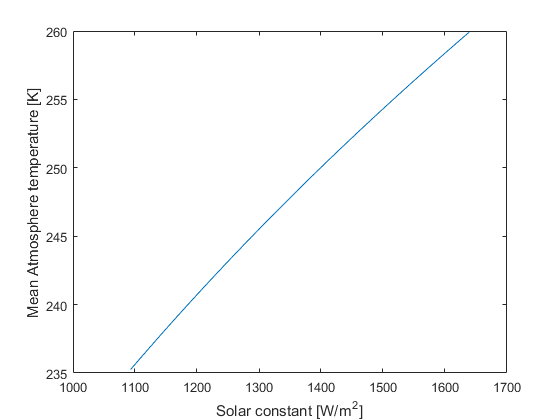
\includegraphics[width=\textwidth]{solar_atm}
		{{\small Relationship between mean atmosphere temperature and solar constant.}}    
	\end{subfigure}
	\begin{subfigure}[b]{0.8\textwidth}   
		\centering 
		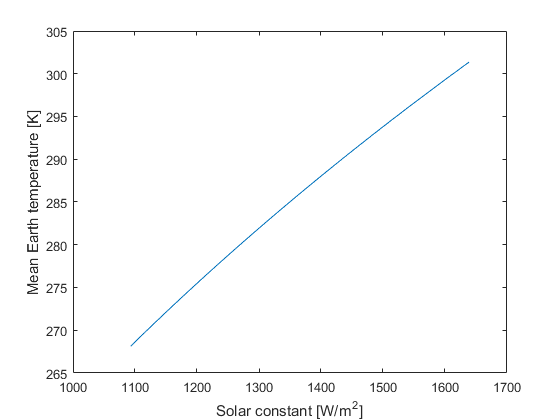
\includegraphics[width=\textwidth]{solar_earth}
		{{\small Relationship between mean Earth's temperature and solar constant.}}    
	\end{subfigure}
\end{figure}

The relationship is linear which makes sense looking at the equation.

\subsection{Comparison of the results}

\subsubsection{Mean Earth Temperature}

\begin{table}[H]
	\centering
	\caption{Comparison between mean Earth's temperature with and without including atmoshere.}
	\label{my-label}
	\begin{tabular}{l|l|l|}
		\cline{2-3}
		& Without Atmosphere       & Including Atmosphere     \\ \hline
		\multicolumn{1}{|l|}{Mean Earth Temperature} & 254.8158\textdegree{K} & 285.9920\textdegree{K} \\ \hline
	\end{tabular}
\end{table}

As seen on the table \ref{my-label} calculated temperature differs for about 30\textdegree{K} which is only around $10\%$ and in the same order of magnitude. In reality it is about 274.15\textdegree{K} so there is no clear advantage of any used method.

\subsubsection{Relationship between mean temperature and solar constant}

In both cases the relationship is linear.

\subsection{Glaciations mechanism}

Now it's time to implement glaciations mechanism in second model. It is very similar to what was done with relationship between mean temperature and solar constant. In fact, it is enough to add one extra condition to the implementation:

\lstinputlisting[language=Matlab, caption = {Glaciations mechanism.}, frame=single]{../source_code/glaciation.m} 

Please note that in this implementation we assume that everything under 269\textdegree{K} is snow and triggers albedo changes. Visualization of the results is presented below:

\begin{figure}[H]
	\centering
	\begin{subfigure}[b]{0.8\textwidth}   
		\centering 
		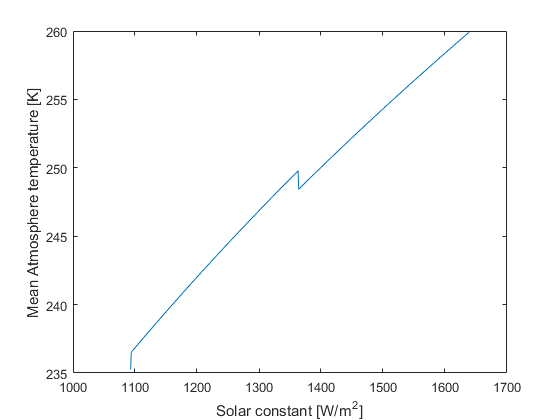
\includegraphics[width=\textwidth]{glac_atm}
		{{\small Relationship between mean atmosphere temperature and solar constant with glaciation mechanism.}}    
	\end{subfigure}
	\begin{subfigure}[b]{0.8\textwidth}   
		\centering 
		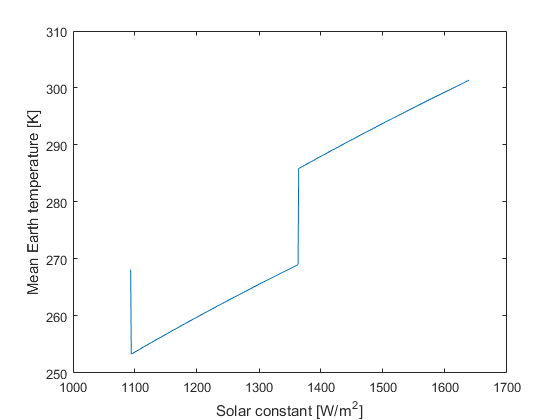
\includegraphics[width=\textwidth]{glac_earth}
		{{\small Relationship between mean Earth's temperature and solar constant with glaciation mechanism.}}    
	\end{subfigure}
\end{figure}

This time relationship is more interesting than simple linear function. Here we see that whenever Earth's temperature goes below given "snow" threshold (269\textdegree{K}) and the snow is slowly melting -- mean atmosphere temperature rises at higher point than without this process for the same solar constant. As soon as higher albedo is reached we observe rapid increase in mean Earth's temperature.

\section{Conclusion}

During this laboratory we have successfully implemented simulation of the global radiation budget of the Earth. We've performed calculations of mean Earth temperature with and without inclusion of temperature acquiring satisfying results in both cases. We've looked at their relationship to solar constant extending model to include glacial-interglacial transition of the Earth system. This allowed us to see how change in albedo can influence mean temperature in both Earth and its atmosphere.

\end{document}
